\documentclass[11pt]{article}

\input{../../preamble.tex}

\usepackage[margin=1in]{geometry}
\usepackage{amsmath, amssymb}
\usepackage{mathtools}
\usepackage{enumitem}


\setlist[itemize]{noitemsep, topsep=2pt}
\setlist[enumerate]{noitemsep, topsep=2pt}

\begin{document}

\begin{center}
{\Large University of British Columbia}\\[4pt]
{\large MECH 464/563 \quad EECE 442/589: Introduction to Robotics / Industrial Robotics}\\[8pt]
{\large \textbf{Homework Assignment \#2.}}\\
{Dominic Klukas}\\
{SN: 64348378}
\end{center}

\vspace{8pt}
Read Ch 1 Math Preliminaries, pp. 13--19.

\vspace{10pt}
\noindent \textbf{Exercise \# 1: (10 marks)} Find the inverse of the following $4\times 4$ matrix, where the $3\times 3$
matrix is a rotation.
\[
\begin{bmatrix}
Q & d\\
0 & 1
\end{bmatrix}
\]


\textbf{Solution.}
We are looking for a matrix $T$ such that
\[
    T \cdot \begin{bmatrix} Q & d \\ 0 & 1 \end{bmatrix}  = I = \begin{bmatrix} Q & d \\ 0 & 1 \end{bmatrix} T
.\] 
Since $Q$ is a rotation matrix, $Q Q^{T} = 1$.
Also, the $1 \times 1$ block matrix has inverse $[1]$.
Therefore, $T$ must have the form
\[
    T = \begin{bmatrix} Q^{T} & x \\ y^{T} & 1 \end{bmatrix} 
\] 
for some vectors $x, y$.
We compute:
\[
    T \cdot \begin{bmatrix} Q & d \\ 0 & 1 \end{bmatrix} = \begin{bmatrix} Q^{T} & x \\ y^{T} & 1 \end{bmatrix} \cdot
\begin{bmatrix} Q & d \\ 0 & 1 \end{bmatrix}=  \begin{bmatrix} I & Q^{T}d + x \\ y^{T}Q & 1 \end{bmatrix} 
.\] 
Then, we require $y^{T} Q = Q^{T} d + x = 0$.
This is the case for an arbitrary rotation matrix $Q$ when $y = 0$ and $x = -Q^{T}d$.
Then, we have:
\[
    T = \begin{bmatrix} Q^{T} & -Q^{T}d \\ 0 & 1 \end{bmatrix} 
.\] 
We check left multiplication:
\[
    \begin{bmatrix} Q & d \\ 0 & 1 \end{bmatrix} \cdot \begin{bmatrix} Q^{T} & -Q^{T}d \\ 0 & 1 \end{bmatrix} = \begin{bmatrix} I & -QQ^{T}d + d \\ 0 & 1 \end{bmatrix} = I
,\] 
as desired.
Therefore,
\[
    \begin{bmatrix} Q & d \\ 0 & 1 \end{bmatrix}^{-1} = \begin{bmatrix} Q^{T} & -Q^{T}d \\ 0& 1  \end{bmatrix} 
.\] 


\vspace{10pt}
\noindent \textbf{Exercise \# 2: (20 marks)}
\begin{enumerate}[label=(\roman*)]
\item A vector product function is specified as
\[
f(x) = \bigl(-2\,\mathbf{i}_0 + 3\,\mathbf{j}_0 - 5\,\mathbf{k}_0\bigr)\times x.
\]
What is the matrix representation of $f$ in $C_0 = [\mathbf{i}_0\ \mathbf{j}_0\ \mathbf{k}_0]$?
What is the matrix representation of $f$ in
\[
C_1 = [\mathbf{i}_1\ \mathbf{j}_1\ \mathbf{k}_1] = [-\mathbf{i}_0\ -\mathbf{j}_0\ \mathbf{k}_0]?
\]

\item What is the coordinate representation ${}^{0}\!Q$ in $C_0$ of a rotation
\[
y = Q(\mathbf{k}_0,\tfrac{\pi}{2})\,x
\]
about axis $\mathbf{k}_0$ of angle $\pi/2$?

\item What is the coordinate representation ${}^{0}\!R$ in $C_0$ of a rotation
\[
y = R(\mathbf{i}_0,\tfrac{\pi}{6})\,x
\]
about axis $\mathbf{i}_0$ of angle $\pi/6$?

\item What is the coordinate representation of the composition of the two rotations
\[
y = R(\mathbf{i}_0,\tfrac{\pi}{6})\,Q(\mathbf{k}_0,\tfrac{\pi}{2})\,x
\]
in $C_0$?

\item Let $C_1$ be the rotated frame $C_1 = Q(\mathbf{k}_0,\tfrac{\pi}{2})\,C_0$.
What is the coordinate representation of the composition of the two rotations
\[
y = R(\mathbf{i}_0,\tfrac{\pi}{6})\,Q(\mathbf{k}_0,\tfrac{\pi}{2})\,x
\]
in $C_1$?
\end{enumerate}

\textbf{Solution}.

\noindent\textbf{Solution.}

\begin{enumerate}[label=(\roman*)]

\item The vector defining the cross product is
\[
{}^{0}\!s = \begin{bmatrix} -2 \\ 3 \\ -5 \end{bmatrix}.
\]
The linear map $f(x)=s\times x$ is represented in $C_0$ by the skew-symmetric matrix
\[
{}^{0}\!f = ({}^{0}\!s)^\times
=
\begin{bmatrix}
0 & 5 & 3\\
-5 & 0 & 2\\
-3 & -2 & 0
\end{bmatrix}.
\]

The change-of-coordinates matrix between $C_0$ and $C_1$ is
\[
{}^{0}\!C_1 = \mathrm{diag}(-1,-1,1), \qquad {}^{1}\!C_0 = ({}^{0}\!C_1)^T = {}^{0}\!C_1.
\]
The representation of the same linear map in $C_1$ is therefore
\[
{}^{1}\!f = {}^{1}\!C_0\;{}^{0}\!f\;{}^{0}\!C_1
=
\begin{bmatrix}
0 & 5 & -3\\
-5 & 0 & -2\\
3 & 2 & 0
\end{bmatrix}.
\]

\item A rotation of angle $\pi/2$ about $\mathbf{k}_0$ has coordinate representation
\[
{}^{0}\!Q =
\begin{bmatrix}
\cos\frac{\pi}{2} & -\sin\frac{\pi}{2} & 0\\
\sin\frac{\pi}{2} & \cos\frac{\pi}{2} & 0\\
0 & 0 & 1
\end{bmatrix}
=
\begin{bmatrix}
0 & -1 & 0\\
1 & 0 & 0\\
0 & 0 & 1
\end{bmatrix}.
\]

\item A rotation of angle $\pi/6$ about $\mathbf{i}_0$ has coordinate representation
\[
{}^{0}\!R =
\begin{bmatrix}
1 & 0 & 0\\
0 & \cos\frac{\pi}{6} & -\sin\frac{\pi}{6}\\
0 & \sin\frac{\pi}{6} & \cos\frac{\pi}{6}
\end{bmatrix}
=
\begin{bmatrix}
1 & 0 & 0\\
0 & \frac{\sqrt{3}}{2} & -\frac{1}{2}\\
0 & \frac{1}{2} & \frac{\sqrt{3}}{2}
\end{bmatrix}.
\]

\item The coordinate representation of the composition $RQ$ in $C_0$ is
\[
{}^{0}\!(RQ) = {}^{0}\!R\;{}^{0}\!Q
=
\begin{bmatrix}
0 & -1 & 0\\
\frac{\sqrt{3}}{2} & 0 & -\frac{1}{2}\\
\frac{1}{2} & 0 & \frac{\sqrt{3}}{2}
\end{bmatrix}.
\]

\item Since $C_1 = Q\,C_0$, we have ${}^{0}\!C_1 = {}^{0}\!Q$ and ${}^{1}\!C_0 = ({}^{0}\!Q)^T$.
Thus the coordinate representation of the same rotation in $C_1$ is
\[
{}^{1}\!(RQ) = {}^{1}\!C_0\;{}^{0}\!(RQ)\;{}^{0}\!C_1
=
\begin{bmatrix}
0 & -\frac{\sqrt{3}}{2} & -\frac{1}{2}\\
1 & 0 & 0\\
0 & -\frac{1}{2} & \frac{\sqrt{3}}{2}
\end{bmatrix}.
\]

\end{enumerate}


\vspace{10pt}
\noindent \textbf{Exercise \# 3 (10 marks)}\\
Find the velocity of a point $\tilde{y}$ with coordinates
\[
y(t) = d(t) + Q(t)\,x(t),
\]
where $Q(t)$ is a rotation matrix, as a function of $\dot d$, $\dot x$ and $\dot Q = \omega \times Q$.
Provide a physical interpretation for each of the terms.
Find the acceleration of a point with coordinates
\[
y(t) = d(t) + Q(t)\,x(t),
\]
where $Q(t)$ is a rotation matrix.


\textbf{Solution.}

We compute:
\[
\dot y (t) = \dot d (t) + \dot Q(t) x(t) + Q(t) \dot x(t) = \dot d (t) + \omega \times  Q(t) x(t) + Q(t) \dot x(t)
.\] 
If $y(t)$ is in frame $C_1$, then let $C_1 = QC_0$. That is, $Q = ^1C_0$.

\begin{itemize}
    \item $\dot x$ is the velocity of the point with respect to the co-ordinate origin $d$ in frame $C_0$
    \item $\omega$ is the angular velocity of frame $C_0$ with respect to frame $C_1$
    \item $\dot d$ is the velocity of frame $C_0$ w.r.t. the frame $C_1$.
\end{itemize}
We compute the acceleration:
\begin{align*}
    \ddot y &= \ddot d + \dot \omega \times Q x + \omega \times  \omega \times Q x + \omega \times  Q \dot x + \omega \times  Q \dot x + Q \ddot x\\
            &= \ddot d + \dot \omega \times Q x + \omega \times  \omega \times Q x + 2\omega \times  Q \dot x + Q \ddot x
.\end{align*}
where we used the fact that $\dot Q = \omega \times  Q$.

\vspace{12pt}
\noindent Only graduate students have to hand in the following two problems:

\vspace{10pt}
\noindent \textbf{Exercise \# 4: (30 marks)}\\
Read the ch1 \texttt{Quaternions2024.pdf} chapter from the Reading Material Canvas Module.\\
Write a Simulink model to integrate
\[
\dot Q = \omega \times Q,\qquad \dot\omega = \tau,\qquad \omega(0)=0,\qquad Q(0)=I,
\]
driven by a specified torque $\tau$.
Animate the motion (block provided in Simulink tutorial, can use a frame or other) whose
coordinate transformation is given by $Q$. This corresponds to your animating a rigid body
having an inertia matrix equal to the identity.
Does the matrix $Q(t)$ remain a rotation matrix for all $t$ as you integrate it?
If not, how would you fix it?

\vspace{6pt}
Provide $Q(t)$ and the animation (or just last image) for the following cases:
\begin{enumerate}[label=(\alph*)]
\item $\tau = [0;\ 0;\ 1]$, $t=5\,\mathrm{s}$;
\item $\tau = [0;\ -1;\ 1]$, $t=8\,\mathrm{s}$;
\item $\tau = [1;\ 1;\ -1]$, $t=4\,\mathrm{s}$.
\end{enumerate}

Write a Simulink block to integrate the quaternion, with the same $\tau$ and $\omega$ as in Exercise \# 3.
Generate the rotation matrix, animate the motion.
How about $q(t)$, does it remain a ``unit'' quaternion?
Propose and implement a method to fix this. Discuss.


\textbf{Solution.}

$Q(t)$ and last image for integrated rotation matrix:

% Preamble:
% \usepackage{graphicx}
% \usepackage{subcaption}

\begin{figure}[htbp]
    \centering

    \begin{subfigure}[t]{0.32\textwidth}
        \centering
        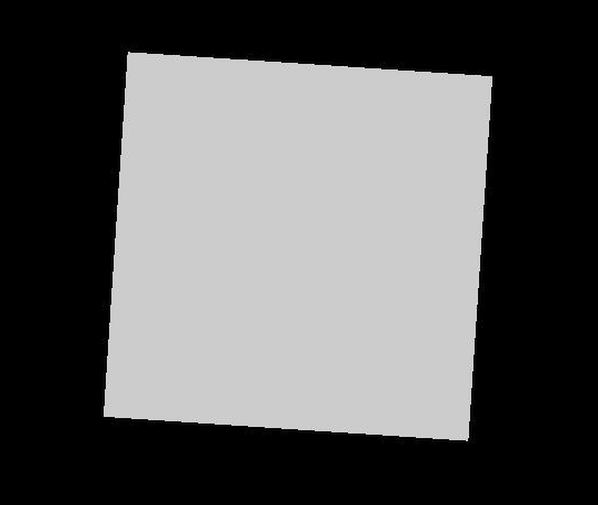
\includegraphics[width=\linewidth]{T1_Rot.png}
        \caption{$t=5\,\mathrm{s}$,\;\;
        $\tau=\begin{bmatrix}0&0&1\end{bmatrix}$}
        \label{fig:T1_Rot}
    \end{subfigure}\hfill
    \begin{subfigure}[t]{0.32\textwidth}
        \centering
        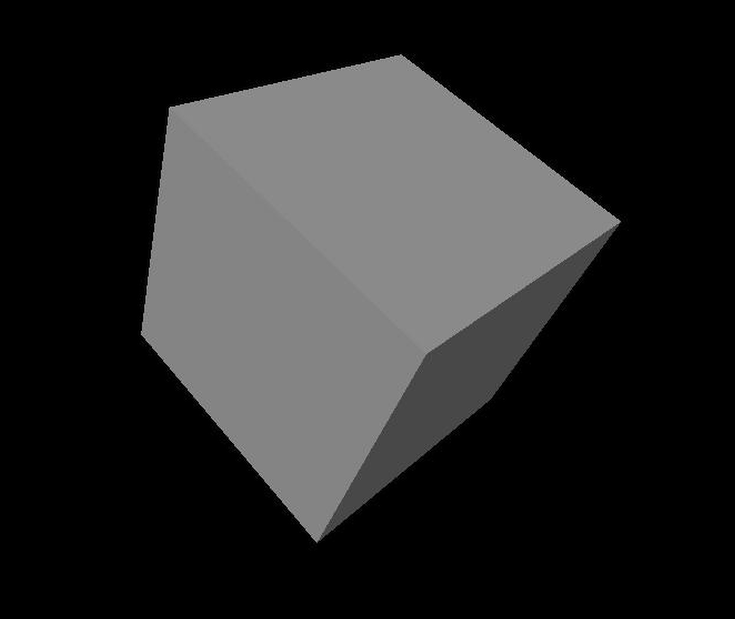
\includegraphics[width=\linewidth]{T2_Rot.png}
        \caption{$t=8\,\mathrm{s}$,\;\;
        $\tau=\begin{bmatrix}0&-1&1\end{bmatrix}$}
        \label{fig:T2_Rot}
    \end{subfigure}\hfill
    \begin{subfigure}[t]{0.32\textwidth}
        \centering
        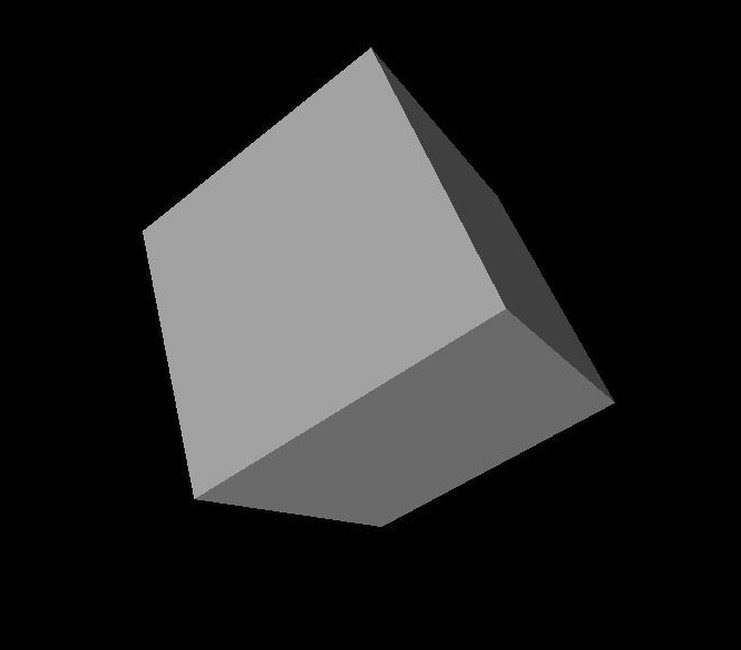
\includegraphics[width=\linewidth]{T3_Rot.png}
        \caption{$t=4\,\mathrm{s}$,\;\;
        $\tau=\begin{bmatrix}1&1&-1\end{bmatrix}$}
        \label{fig:T3_Rot}
    \end{subfigure}

    \caption{Rigid-body orientation using rotation-matrix integration (\(Q\)-integration).}
    \label{fig:RotRow}
\end{figure}

\begin{figure}[htbp]
    \centering

    \begin{subfigure}[t]{0.32\textwidth}
        \centering
        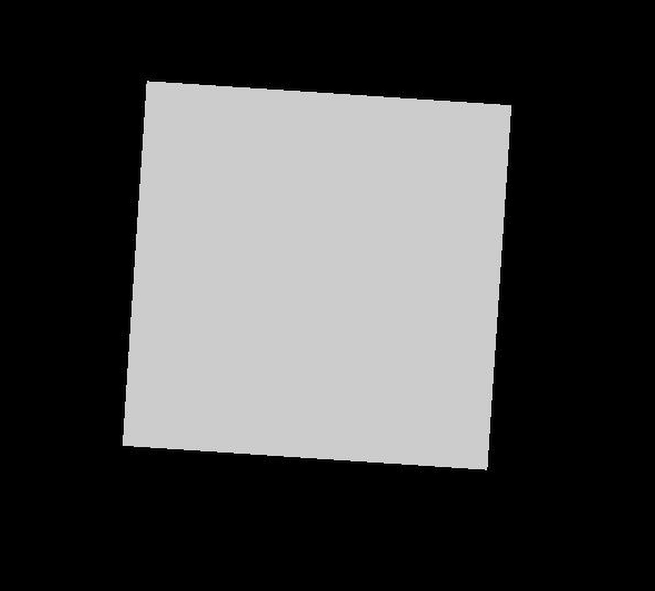
\includegraphics[width=\linewidth]{T1_Quat.png}
        \caption{$t=5\,\mathrm{s}$,\;\;
        $\tau=\begin{bmatrix}0&0&1\end{bmatrix}$}
        \label{fig:T1_Quat}
    \end{subfigure}\hfill
    \begin{subfigure}[t]{0.32\textwidth}
        \centering
        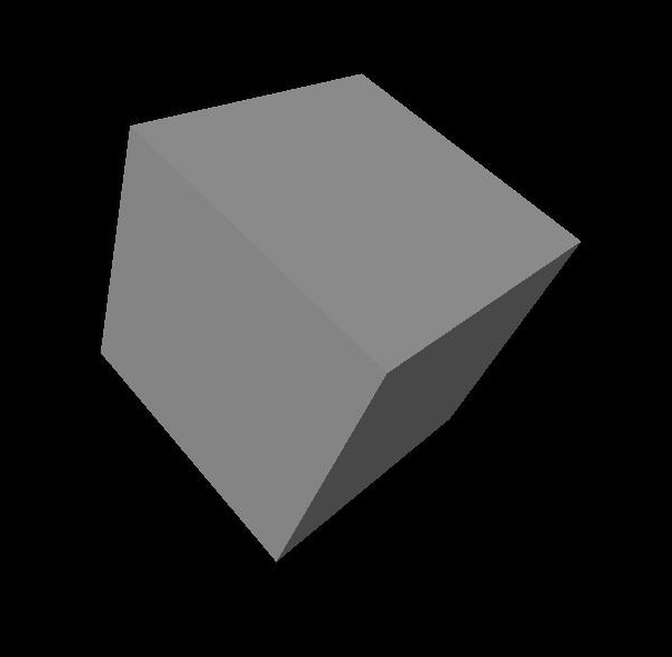
\includegraphics[width=\linewidth]{T2_Quat.png}
        \caption{$t=8\,\mathrm{s}$,\;\;
        $\tau=\begin{bmatrix}0&-1&1\end{bmatrix}$}
        \label{fig:T2_Quat}
    \end{subfigure}\hfill
    \begin{subfigure}[t]{0.32\textwidth}
        \centering
        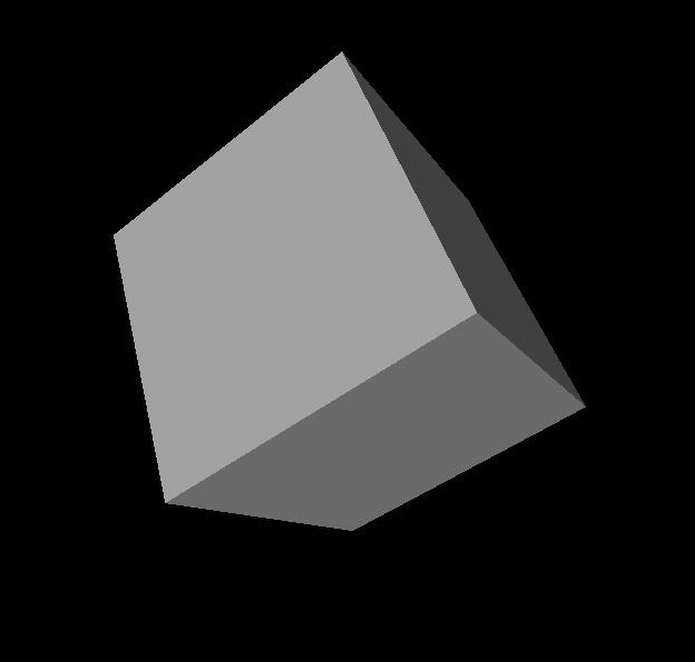
\includegraphics[width=\linewidth]{T3_Quat.png}
        \caption{$t=4\,\mathrm{s}$,\;\;
        $\tau=\begin{bmatrix}1&1&-1\end{bmatrix}$}
        \label{fig:T3_Quat}
    \end{subfigure}

    \caption{Rigid-body orientation using quaternion integration with normalization.}
    \label{fig:QuatRow}
\end{figure}

\begin{enumerate}
\item[(a)]
$\tau=\begin{bmatrix}0&0&1\end{bmatrix}$, \quad $t=5\,\mathrm{s}$.
\[
Q(5)=
\begin{bmatrix}
0.9978 & 0.0663 & 0\\
-0.0663 & 0.9978 & 0\\
0 & 0 & 1.0000
\end{bmatrix}
\]
\[
q(5)=0.9994 + 0\,i + 0\,j - 0.0332\,k
\]
\[
R\!\left(q(5)\right)\approx
\begin{bmatrix}
0.9978 & 0.0664 & 0\\
-0.0664 & 0.9978 & 0\\
0 & 0 & 1.0000
\end{bmatrix}
\]

\item[(b)]
$\tau=\begin{bmatrix}0&-1&1\end{bmatrix}$, \quad $t=8\,\mathrm{s}$.
\[
Q(8)=
\begin{bmatrix}
0.2902 & -0.6760 & -0.6760\\
0.6760 & 0.6451 & -0.3549\\
0.6760 & -0.3549 & 0.6451
\end{bmatrix}
\]
\[
q(8)= -0.8043 + 0\,i + 0.4202\,j - 0.4202\,k
\]
\[
R\!\left(q(8)\right)\approx
\begin{bmatrix}
0.2938 & -0.6759 & -0.6759\\
0.6759 & 0.6469 & -0.3531\\
0.6759 & -0.3531 & 0.6469
\end{bmatrix}
\]

\item[(c)]
$\tau=\begin{bmatrix}1&1&-1\end{bmatrix}$, \quad $t=4\,\mathrm{s}$.
\[
Q(4)=
\begin{bmatrix}
0.5180 & 0.7957 & 0.3137\\
-0.3137 & 0.5180 & -0.7957\\
-0.7957 & 0.3137 & 0.5180
\end{bmatrix}
\]
\[
q(4)=0.7991 + 0.3471\,i + 0.3471\,j - 0.3471\,k
\]
\[
R\!\left(q(4)\right)\approx
\begin{bmatrix}
0.5181 & 0.7957 & 0.3138\\
-0.3138 & 0.5181 & -0.7957\\
-0.7957 & 0.3138 & 0.5181
\end{bmatrix}
\]
\end{enumerate}


The matrix $Q(t)$ does not remain a rotation matrix for all $t$ as you integrate it because of numerical error in the integration. We can confirm this pretty easily: indeed, a rotation matrix has the property that $Q \cdot Q^T = I$. But, for $Q(5)$ in part a), we have
\[
    Q(5)(Q(5))^{T} = \begin{bmatrix} 1.00000053 & 0 & 0\\ 0 & 1.00000053 & 0\\ 0 & 0 & 1 \end{bmatrix} \neq I
.\] 
Therefore, $Q(5)$ is not a perfect rotation matrix.
This could be rectified by making the singular values of the matrix 1.
If we take the SVD composition of $Q$, we will get $Q = U\Sigma V^{T}$.
$U$ and $V^{T}$ are orthonormal matrices, and $\Sigma$ will be a diagonal matrix with singular values being close to 1, accounting for the error.
If we reset the singular values all to 1, then $Q_{fixed} = UV^{T}$ will be an orthogonal matrix.

$q(t)$ also does not remain a "unit" quaternion, because of numerical integration errors.
Indeed, we can compute $q(5)q(5)^{*} =0.99990260 \neq 1$.
In order to rectify this, we can normalize the quaternion after each integration.

\begin{figure}[htbp]
    \centering
    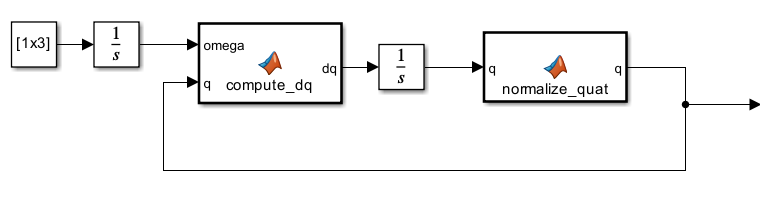
\includegraphics[width=0.95\linewidth]{Normalization.png}
    \caption{Simulink Block to integrate and normalize quaternion, so that quaternion remains a "unit" rotation quaternion}
    \label{fig:quat_normalization}
\end{figure}
The code block in "normalize\_quat" simply computes $q = q / \|q\|$.


\vspace{10pt}
\noindent \textbf{Exercise \# 5: (20 marks)}
\begin{enumerate}[label=(\alph*)]
\item Show that for any $x \in \mathbb{R}^4$,
\[
x^{T} e^{\theta(\hat{s}^{\circ})} x = \cos\theta\,\|x\|^2,
\]
where $e^{\theta(\hat{s}^{\circ})}$ is as given in equation (34), p. 6 of the quaternion handout.

\item Consider the function $f:\mathbb{R}^4\to\mathbb{R}^4$ defined by the quaternion product
\[
f(x)=(d+a\mathbf{i})\,x\,(d+a\mathbf{i})^{-1}
\]
(or in vector form $(d+a\mathbf{i})\circ (d x+ v_x)\circ (d+a\mathbf{i})^{-1}$,
similarly to eq (45) p. 9 of the notes on Quaternions, but with $x$ and $f(x)$ in $\mathbb{R}^4$).
Also define
\[
f_\ell(x)=(d+a\mathbf{i})x,\qquad f_r(x)=x(d+a\mathbf{i})^{-1},\qquad f_\ell,f_r:\mathbb{R}^4\to\mathbb{R}^4.
\]
Clearly $f_\ell$, $f_r$, and $f$ are linear. Find their matrix representations.
What do each of these functions represent, geometrically?
\end{enumerate}


\textbf{Solution.}
\begin{enumerate}
    \item We are given that
        \[
            e^{\theta (\hat s \circ)} = \cos \theta I + \sin \theta \begin{bmatrix} 0 & - \hat{s}^{T} \\ \hat{s} & \hat{s} \times  \end{bmatrix}
        .\] 
        Write $x = [x_0 \ \hat{x}]^{T}$ where $\hat{x} = [x_1 \  x_2\  x_3]^{T}$.
        Then, we compute:
        \begin{align*}
             x^T e^{\theta (\hat s \circ)} x &=  x^{T}(\cos \theta I + \sin \theta \begin{bmatrix} 0 & - \hat{s}^{T} \\ \hat{s} & \hat{s} \times  \end{bmatrix})x\\
                                             &=\cos \theta x^{T} x + \sin \theta x^{T}\begin{bmatrix} 0 & - \hat{s}^{T} \\ \hat{s} & \hat{s} \times  \end{bmatrix}x\\
                                            &= \cos \theta \|x\|^2 + \sin \theta x^T \begin{bmatrix} -\hat s^T \hat x\\ x_0 \hat s + \hat s \times \hat x \end{bmatrix} \\
                                            &= \cos \theta \|x\|^2 + \sin \theta \left( -x_0 \hat s^T \hat x + \hat x^T (x_0 \hat s) + \hat x^T \hat s \times \hat x \right) 
        .\end{align*}
        However, $\hat x^T \hat s \times \hat x = 0$ since $\hat x^T$ and $\hat s \times  \hat x $ are perpendicular so their dot product is zero.
        Also, $-x_0 \hat s^T \hat x + \hat x^T (x_0 \hat s) = 0$. Thus, the $\sin\theta$ term is zero so we get $x^T e^{\theta (\hat s \circ)} x = \cos \theta \|x\|^2$.
    \item 
        First, we interpret a vector $x \in \mathbb{R}^{4}$ as $[x_0\ x_1\ x_2\ x_3] = x_0 + x_1i + x_2j + x_3k$.
        Also, we recall that $(d+ai)^{-1} = \frac{1}{d^2 + a^2} [d - ai]$.
        Then,
        \begin{align*}
            f_l (x) &= (d + ai) (x_0 + x_1i + x_2j + x_3k) \\
            &= (dx_0 - ax_1) + (dx_1 + ax_0) i + (dx_2 - ax_3) j + (dx_3 + a_2 x_2) k \\
            &= \begin{bmatrix} d & -a & 0 & 0\\ a & d & 0 & 0 \\ 0 & 0 & d & -a \\ 0 & 0 & a & d \end{bmatrix} \cdot \begin{bmatrix} x_0 \\ x_1 \\ x_2 \\ x_3 \end{bmatrix}\\
            &=  \sqrt{a^2 + d^2}\begin{bmatrix} \frac{d}{\sqrt{a^2 + d^2}} & -\frac{a}{\sqrt{a^2 + d^2}} & 0 & 0\\ \frac{a}{\sqrt{a^2 + d^2}} & \frac{d}{\sqrt{a^2 + d^2}} & 0 & 0 \\ 0 & 0 & \frac{d}{\sqrt{a^2 + d^2}} & -\frac{a}{\sqrt{a^2 + d^2}} \\ 0 & 0 & \frac{a}{\sqrt{a^2 + d^2}} & \frac{d}{\sqrt{a^2 + d^2}} \end{bmatrix} \cdot \begin{bmatrix} x_0 \\ x_1 \\ x_2 \\ x_3 \end{bmatrix}\\
        \end{align*}
        In this form, we can see that this matrix performs two rotations, in the $i_0, i_1$ and $i_2, i_3$ planes respectively, both "counter-clockwise" by angle $\theta = \cos^{-1}(d / \sqrt{a^2 + d^2})$, and scales the rotated vector by $\sqrt{a^2 + d^2}$.

        Similarly,
        \begin{align*}
            f_r (x) &= (x_0 + x_1i + x_2 j + x_3k) \cdot \frac{1}{d^2 + a^2} (d - ai) \\
            &= \frac{1}{d^2 + a^2} ((x_0 d + a x_1) + (d x_1 - a x_0) i + (d x_2 - ax_3)j + (d x_3 + a x_2)k) \\
            &= \frac{1}{d^2 + a^2} \begin{bmatrix} d & a & 0 & 0 \\ -a & d & 0 & 0 \\ 0 & 0 & d & -a\\ 0 & 0 & a & d \end{bmatrix} \cdot \begin{bmatrix} x_0 \\ x_1 \\ x_2 \\ x_3 \end{bmatrix} \\
            &= \frac{1}{\sqrt{d^2 + a^2}} \begin{bmatrix} \frac{d}{\sqrt{a^2 + d^2}} & \frac{a}{\sqrt{a^2 + d^2}} & 0 & 0 \\ -\frac{a}{\sqrt{a^2 + d^2}} & \frac{d}{\sqrt{a^2 + d^2}} & 0 & 0 \\ 0 & 0 & \frac{d}{\sqrt{a^2 + d^2}} & -\frac{a}{\sqrt{a^2 + d^2}}\\ 0 & 0 & \frac{a}{\sqrt{a^2 + d^2}} & \frac{d}{\sqrt{a^2 + d^2}} \end{bmatrix} \cdot \begin{bmatrix} x_0 \\ x_1 \\ x_2 \\ x_3 \end{bmatrix} 
        .\end{align*}
        We likewise recognize this as a linear map that performs a clockwise rotation in the plane $i_0, i_1$, and a counter-clockiwse rotation in the plane $i_2, i_3$, both by angle $\theta = \cos^{-1} (d / \sqrt{a^2 + d^2})$.

        Then, we compute $f = f_l \cdot f_r$.
        \[
            f = \frac{1}{a^2 + d^2} \begin{bmatrix} a^2 + d^2 & 0 & 0 & 0 \\ 0 & a^2 + d^2 & 0 & 0 \\ 0 & 0 & d^2 - a^2 & -2ad \\ 0 & 0 & 2ad & d^2 - a^2 \end{bmatrix}  = \begin{bmatrix} 1 & 0 & 0 & 0 \\ 0 & 1 & 0 & 0 \\ 0 & 0 & \frac{d^2 - a^2}{d^2 + a^2} & \frac{-2ad}{d^2 + a^2} \\ 0 & 0 & \frac{2ad}{d^2 + a^2} & \frac{d^2 - a^2}{d^2 + a^2} \end{bmatrix} 
        .\]

Geometric interpretation: We recognize the trig identities: $\cos (2\theta) = \cos^2 \theta - \sin^2 \theta$, and $\sin(2\theta) = 2 \sin\theta \cos\theta$.
        Then, if $\cos\theta = \frac{d}{\sqrt{a^2 + d^2}}$, we have $\cos (2\theta) = \frac{d^2 - a^2}{\sqrt{a^2 + d^2}^2}$ and $\sin(2 \theta) = \frac{2ad}{d^2 + a^2}$.
        Therefore, this matrix performs the identity in the plane defined by $i_0, i_1$, and a rotation by $2 \cos^{-1}(d / \sqrt{a^2 + d^2})$ in the counter-clockwise direction.

\end{enumerate}

\end{document}

